\documentclass{beamer}
\usetheme{Madrid}
\usecolortheme{dolphin}
\usepackage{tikz}
\usepackage{amsmath,amssymb}
\usepackage{algorithm}
\usepackage{algpseudocode}
\usepackage{float}  % for [H]
\usepackage{boxedminipage}
\usepackage{rotating}


%\usepackage{algorithmic}
\usepackage{booktabs}

\title[Minimum Spanning Trees]{Minimum Spanning Trees \& Kruskal's Algorithm}
\author{Lecture Notes}
\date{\today}

\begin{document}

\begin{frame}
\titlepage
\end{frame}

\begin{frame}{Outline}
\tableofcontents
\end{frame}

\section{Youtube Video}

\begin{frame}{Video}
Start by watching this video:

\url{https://www.youtube.com/watch?v=Yldkh0aOEcg&ab_channel=SpanningTree}

\textbf{How Do You Calculate a Minimum Spanning Tree?} by Spanning Tree
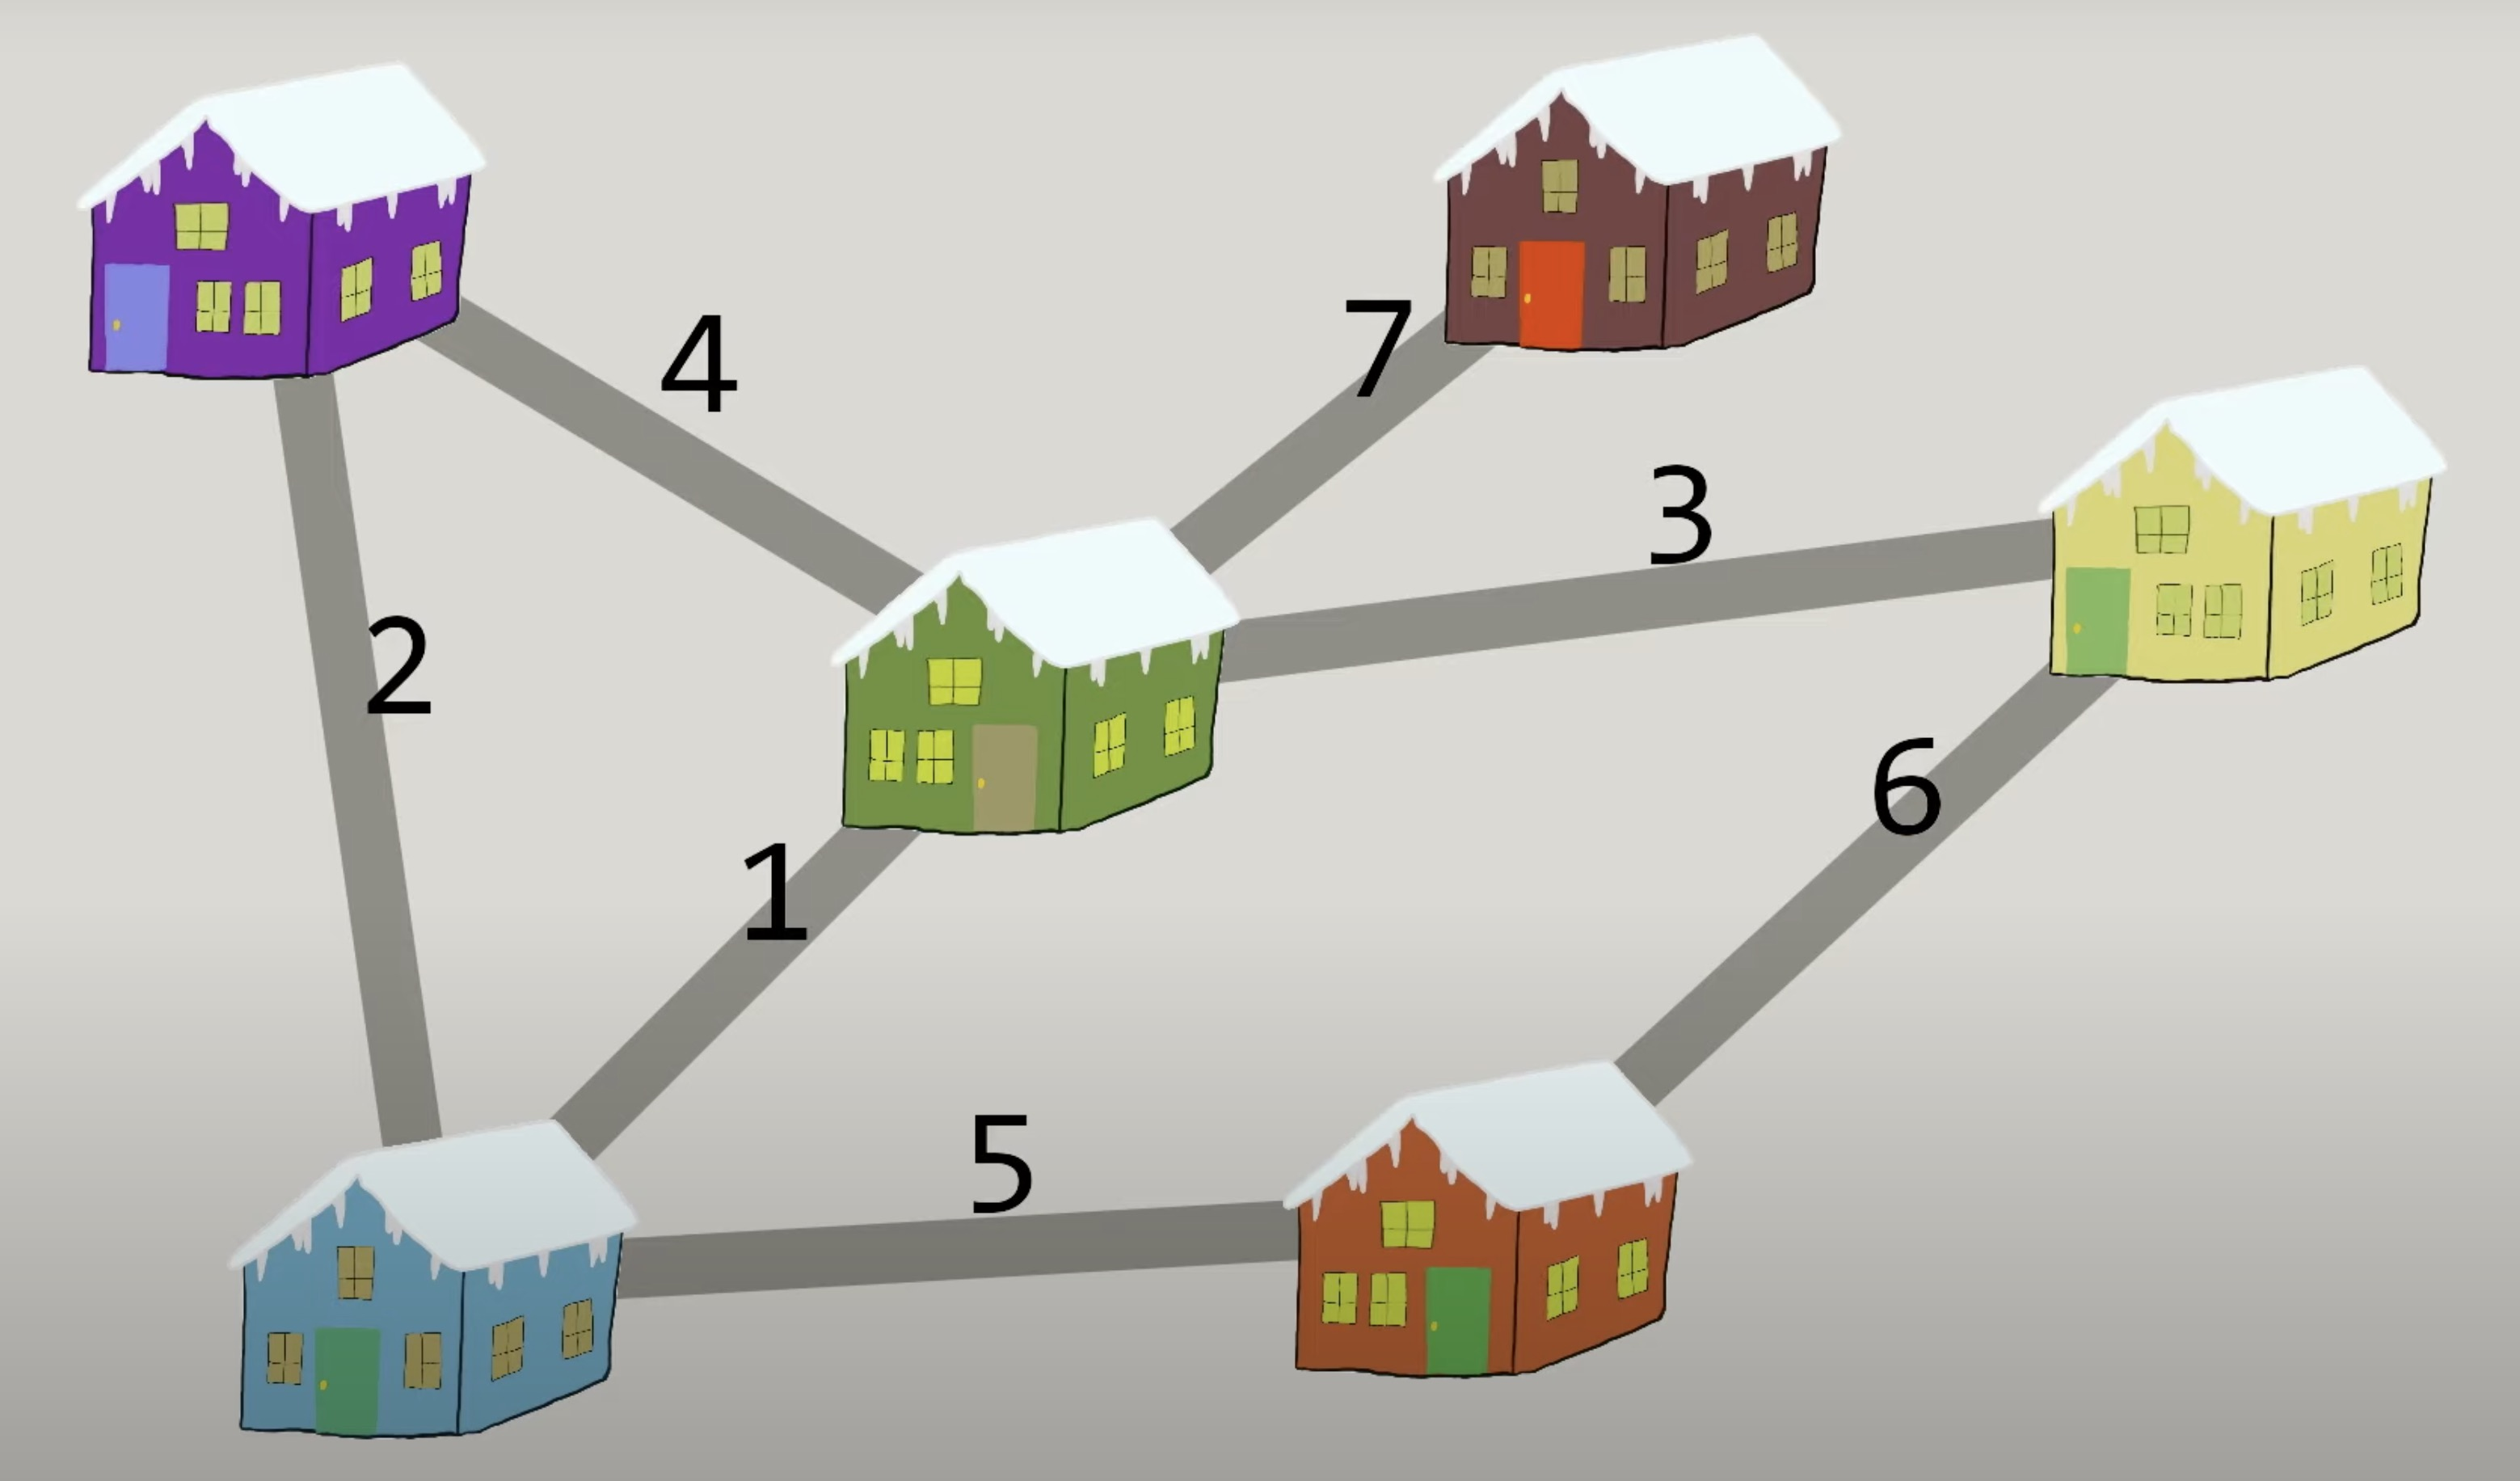
\includegraphics[scale = 0.07]{kruskal-video}
\end{frame}

\section{Spanning Trees}

\begin{frame}{Spanning Trees}
\begin{block}{Definition: Spanning Tree}
A \textbf{spanning tree} is a connected graph using all vertices in which there are no circuits.
\end{block}

\begin{itemize}
\item There is a path from any vertex to any other vertex
\item No circuits (cycles)
\item When we have a weighted graph, we often want the \textbf{minimum cost spanning tree}
\end{itemize}

\begin{center}
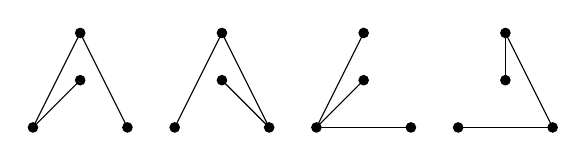
\begin{tikzpicture}[scale=0.6]
% Four examples of spanning trees
\begin{scope}[xshift=0cm]
\draw[fill] (0,0) circle[radius=.1];
\draw[fill] (1,1) circle[radius=.1];
\draw[fill] (1,2) circle[radius=.1];
\draw[fill] (2,0) circle[radius=.1];
\draw(0,0)--(1,2);
\draw(0,0)--(1,1);
\draw(1,2)--(2,0);
\end{scope}

\begin{scope}[xshift=3cm]
\draw[fill] (0,0) circle[radius=.1];
\draw[fill] (1,1) circle[radius=.1];
\draw[fill] (1,2) circle[radius=.1];
\draw[fill] (2,0) circle[radius=.1];
\draw(0,0)--(1,2);
\draw(2,0)--(1,1);
\draw(1,2)--(2,0);
\end{scope}

\begin{scope}[xshift=6cm]
\draw[fill] (0,0) circle[radius=.1];
\draw[fill] (1,1) circle[radius=.1];
\draw[fill] (1,2) circle[radius=.1];
\draw[fill] (2,0) circle[radius=.1];
\draw(0,0)--(1,2);
\draw(0,0)--(1,1);
\draw(0,0)--(2,0);
\end{scope}

\begin{scope}[xshift=9cm]
\draw[fill] (0,0) circle[radius=.1];
\draw[fill] (1,1) circle[radius=.1];
\draw[fill] (1,2) circle[radius=.1];
\draw[fill] (2,0) circle[radius=.1];
\draw(1,1)--(1,2);
\draw(1,2)--(2,0);
\draw(0,0)--(2,0);
\end{scope}
\end{tikzpicture}
\end{center}
\end{frame}

\begin{frame}{Key Property of Spanning Trees}
\begin{block}{Lemma: Number of Edges in a Spanning Tree}
Let $G = (V, E)$ be a connected undirected graph with $|V| = n$ vertices. \\
Then every spanning tree of $G$ contains exactly $???$ edges.
\end{block}

\begin{center}
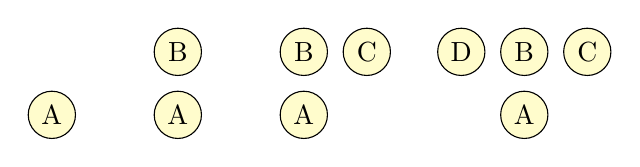
\begin{tikzpicture}[scale=0.8, every node/.style={circle, draw, fill=yellow!20, minimum size=6mm, inner sep=1pt}]
% Examples for n = 1, 2, 3, 4, 5
\node (A1) at (0,0) {A};

% n = 2
\begin{scope}[xshift=2cm]
\node (A2) at (0,0) {A};
\node (B2) at (0,1) {B};

\end{scope}

% n = 3
\begin{scope}[xshift=4cm]
\node (A3) at (0,0) {A};
\node (B3) at (0,1) {B};
\node (C3) at (1,1) {C};

\end{scope}

% n = 4
\begin{scope}[xshift=7.5cm]
\node (A4) at (0,0) {A};
\node (B4) at (0,1) {B};
\node (C4) at (1,1) {C};
\node (D4) at (-1,1) {D};

\end{scope}
\end{tikzpicture}
\end{center}

For $n$ vertices, we need exactly $????$ edges to:
\begin{itemize}
\item Ensure connectivity (must have at least $???$ edges)
\item Avoid cycles (must have at most $???$ edges)
\end{itemize}
\end{frame}

\begin{frame}{Key Property of Spanning Trees}
\begin{block}{Lemma: Number of Edges in a Spanning Tree}
Let $G = (V, E)$ be a connected undirected graph with $|V| = n$ vertices. \\
Then every spanning tree of $G$ contains exactly $n - 1$ edges.
\end{block}

\begin{center}
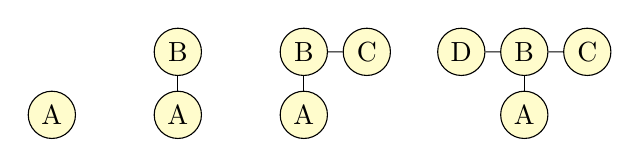
\begin{tikzpicture}[scale=0.8, every node/.style={circle, draw, fill=yellow!20, minimum size=6mm, inner sep=1pt}]
% Examples for n = 1, 2, 3, 4, 5
\node (A1) at (0,0) {A};

% n = 2
\begin{scope}[xshift=2cm]
\node (A2) at (0,0) {A};
\node (B2) at (0,1) {B};
\draw (A2) -- (B2);
\end{scope}

% n = 3
\begin{scope}[xshift=4cm]
\node (A3) at (0,0) {A};
\node (B3) at (0,1) {B};
\node (C3) at (1,1) {C};
\draw (A3) -- (B3);
\draw (B3) -- (C3);
\end{scope}

% n = 4
\begin{scope}[xshift=7.5cm]
\node (A4) at (0,0) {A};
\node (B4) at (0,1) {B};
\node (C4) at (1,1) {C};
\node (D4) at (-1,1) {D};
\draw (A4) -- (B4);
\draw (B4) -- (C4);
\draw (B4) -- (D4);
\end{scope}
\end{tikzpicture}
\end{center}

For $n$ vertices, we need exactly $n-1$ edges to:
\begin{itemize}
\item Ensure connectivity (must have at least $n-1$ edges)
\item Avoid cycles (must have at most $n-1$ edges)
\end{itemize}
\end{frame}
\begin{frame}{Cycles with more than $n-1$ edges}

\end{frame}

\section{Minimum Cost Spanning Tree}

\begin{frame}{Minimum Cost Spanning Tree (MCST)}
\begin{block}{Definition: Minimum Cost Spanning Tree}
The minimum cost spanning tree is the spanning tree with the smallest total edge weight.
\end{block}

\textbf{Practical Problem:} A company needs to lease dedicated lines between their five offices (A, B, C, D, and E). The costs (in thousands of dollars per year) are shown in the graph.

%\vspace{0.3cm}
\begin{center}
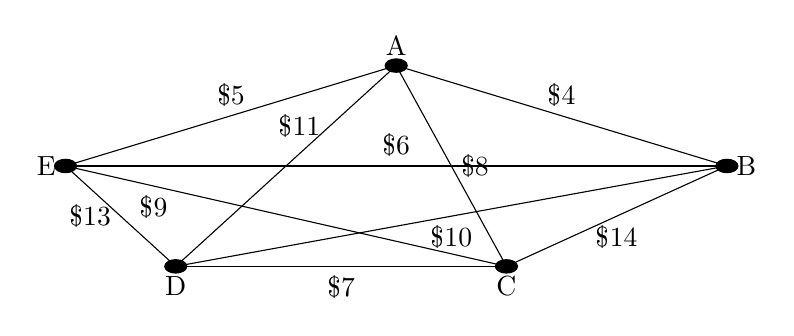
\begin{tikzpicture}[yscale=0.85, xscale = 1.4]
\draw[fill] (0,0) circle[radius=.1] node[below]{D};
\draw[fill] (3,0) circle[radius=.1] node[below]{C};
\draw[fill] (-1,1.5) circle[radius=.1] node[left]{E};
\draw[fill] (2,3) circle[radius=.1] node[above]{A};
\draw[fill] (5,1.5) circle[radius=.1] node[right]{B};
\draw(0,0)--(3,0) node[midway, below]{\$7};
\draw(0,0)--(2,3) node[pos = 0.7, left]{\$11};
\draw(0,0)--(-1,1.5) node[midway, left]{\$13};
\draw(0,0)--(5,1.5) node[midway, below]{\$10};
\draw(3,0)--(-1,1.5) node[pos=0.8, below]{\$9};
\draw(3,0)--(2,3) node[midway, right]{\$8};
\draw(3,0)--(5,1.5) node[midway, below]{\$14};
\draw(-1,1.5)--(2,3) node[midway, above]{\$5};
\draw(-1,1.5)--(5,1.5) node[midway, above]{\$6};
\draw(2,3)--(5,1.5) node[midway, above]{\$4};
\end{tikzpicture}
\end{center}

\textbf{Goal:} Find the smallest set of edges that connects all offices while minimizing total cost.
\end{frame}

\begin{frame}{Applications of MCST}
\begin{enumerate}
    \item \textbf{Network Design:} Connecting cities with fiber optic cables, water pipes, or electrical wires at minimum cost.
    
    \item \textbf{Transportation Infrastructure:} Connecting towns with roads while minimizing construction costs.
    
    \item \textbf{Clustering in Machine Learning:} Capturing data structure through pairwise distances.
    
    \item \textbf{Communication Networks:} Ensuring connectivity between devices with minimal wiring cost.
    
    \item \textbf{Approximation Algorithms:} Used as a subroutine in algorithms for NP-hard problems (e.g., Traveling Salesperson Problem).
\end{enumerate}
\end{frame}

\section{Kruskal's Algorithm}

\begin{frame}{Kruskal's Algorithm}
\begin{block}{Key Idea}
Build a spanning tree by \textbf{\emph{greedily}} adding edges one at a time in order of increasing weight, skipping any edge that would create a cycle.
\end{block}
\vspace{-0.2cm}
\begin{algorithm}[H]
\caption{Kruskal's Algorithm}
\begin{algorithmic}[1]
\State \textbf{Input:} A connected, undirected graph $G = (V, E)$ with edge weights $w(e)$.
\State \textbf{Initialization:} Mark all edges as unused. Set $T \gets \emptyset$.
\Repeat
  \State Select the cheapest unused edge in the graph.
  \If{adding the edge would create a cycle}
    \State Skip this edge.
  \Else
    \State Add the edge to $T$.
  \EndIf
\Until{$T$ contains $|V| - 1$ edges (i.e., a spanning tree has been formed).}
\State \textbf{Output:} The set $T$, forming a minimum spanning tree of $G$.
\end{algorithmic}
\end{algorithm}
\end{frame}

\begin{frame}
\begin{center}
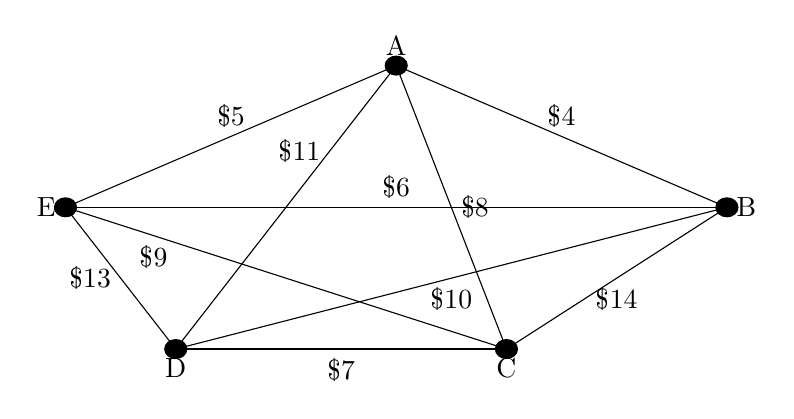
\begin{tikzpicture}[yscale=1.2, xscale = 1.4]
\draw[fill] (0,0) circle[radius=.1] node[below]{D};
\draw[fill] (3,0) circle[radius=.1] node[below]{C};
\draw[fill] (-1,1.5) circle[radius=.1] node[left]{E};
\draw[fill] (2,3) circle[radius=.1] node[above]{A};
\draw[fill] (5,1.5) circle[radius=.1] node[right]{B};
\draw(0,0)--(3,0) node[midway, below]{\$7};
\draw(0,0)--(2,3) node[pos = 0.7, left]{\$11};
\draw(0,0)--(-1,1.5) node[midway, left]{\$13};
\draw(0,0)--(5,1.5) node[midway, below]{\$10};
\draw(3,0)--(-1,1.5) node[pos=0.8, below]{\$9};
\draw(3,0)--(2,3) node[midway, right]{\$8};
\draw(3,0)--(5,1.5) node[midway, below]{\$14};
\draw(-1,1.5)--(2,3) node[midway, above]{\$5};
\draw(-1,1.5)--(5,1.5) node[midway, above]{\$6};
\draw(2,3)--(5,1.5) node[midway, above]{\$4};
\end{tikzpicture}
\end{center}

\footnotesize
\begin{tabular}{|c|c|c|c|c|}
\hline
\textbf{Step} & \textbf{Edge Considered} & \textbf{Forms Cycle?}&\textbf{Add to T?} & \textbf{Cost}\\
\hline
1 &  && & \\
\hline
2 &  &  &&\\
\hline
3 &  &  &&\\
\hline
4 &  &  &&\\
\hline
5 &  & && \\
\hline
6 &  & && \\
\hline
7 &  & && \\
\hline
8 &  & && \\
\hline
9 &  &  &&\\
\hline
\end{tabular}


\end{frame}



\begin{frame}{Example: Company Phone Lines}
Using Kruskal's algorithm for the phone line example:\\

\begin{columns}
\begin{column}{0.5\textwidth}
\begin{tabular}{lll}
AB & \$4 & OK \\
AE & \$5 & OK \\
BE & \$6 & reject -- closes circuit ABEA \\
DC & \$7 & OK \\
AC & \$8 & OK \\
\end{tabular}

\vspace{0.2cm}
Total cost: \$24,000 per year
\end{column}

\begin{column}{0.5\textwidth}
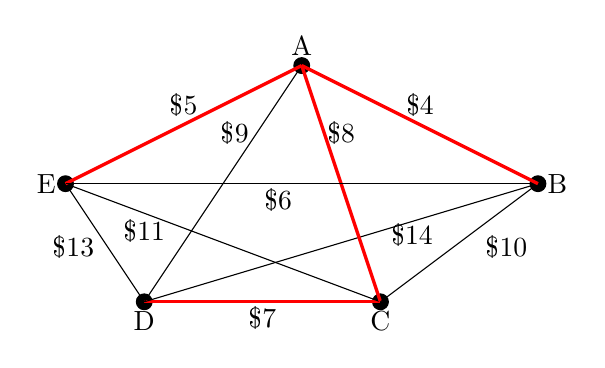
\begin{tikzpicture}{scale = 0.4}
\draw[fill] (0,0) circle[radius=.1] node[below]{D};
\draw[fill] (3,0) circle[radius=.1] node[below]{C};
\draw[fill] (-1,1.5) circle[radius=.1] node[left]{E};
\draw[fill] (2,3) circle[radius=.1] node[above]{A};
\draw[fill] (5,1.5) circle[radius=.1] node[right]{B};
\draw[very thick, red](0,0)--(3,0);
\draw(0,0)--(2,3);
\draw(0,0)--(-1,1.5);
\draw(0,0)--(5,1.5);
\draw(3,0)--(-1,1.5);
\draw[very thick, red](3,0)--(2,3);
\draw(3,0)--(5,1.5);
\draw[very thick, red](-1,1.5)--(2,3);
\draw(-1,1.5)--(5,1.5);
\draw[very thick, red](2,3)--(5,1.5);
\node at (1.5, -0.2){\$7};
\node at (-0.9, 0.7){\$13};
\node at (4.6,0.7){\$10};
\node at (3.5, 2.5){\$4};
\node at (0.5,2.5){\$5};
\node at (1.7,1.3){\$6};
\node at (1.15,2.15){\$9};
\node at (2.5,2.15){\$8};
\node at (0,0.9){\$11};
\node at (3.4,0.85){\$14};
\end{tikzpicture}
\end{column}
\end{columns}

\begin{itemize}
\item Selected edges form a spanning tree (shown in red)
\item All vertices are connected with no cycles
\item We have $n-1 = 4$ edges for 5 vertices
\item Total cost is minimized
\end{itemize}
\end{frame}

\begin{frame}
\begin{center}
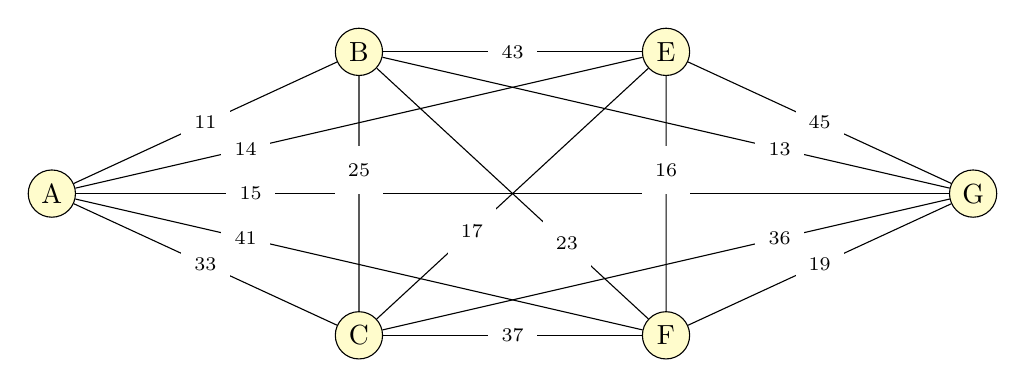
\begin{tikzpicture}[
  yscale=0.6, xscale = 1.3,
  every node/.style={circle, draw, fill=yellow!20, minimum size=6mm, inner sep=1pt},
  edge label/.style={font=\scriptsize, rectangle, draw = white, fill=white, inner sep=2pt}
]

% Nodes
\node (A) at (0,0) {A};
\node (B) at (3,3) {B};
\node (C) at (3,-3) {C};
\node (E) at (6,3) {E};
\node (F) at (6,-3) {F};
\node (G) at (9,0) {G};

% Edges with separate edge label style
\draw (A) -- (B) node[midway, edge label] {11};
\draw (A) -- (C) node[midway, edge label] {33};
\draw (A) -- (E) node[pos=0.3, edge label] {14};
\draw (A) -- (F) node[pos=0.3, edge label] {41};
\draw (A) -- (G) node[pos=0.2, edge label] {15};

\draw (B) -- (C) node[pos=0.4, edge label] {25};
\draw (B) -- (E) node[midway, edge label] {43};
\draw (B) -- (F) node[pos=0.7, edge label] {23};
\draw (B) -- (G) node[pos=0.7, edge label] {13};

\draw (C) -- (E) node[pos=0.35, edge label] {17};
\draw (C) -- (F) node[midway, edge label] {37};
\draw (C) -- (G) node[pos=0.7, edge label] {36};

\draw (E) -- (F) node[pos=0.4, edge label] {16};
\draw (E) -- (G) node[midway, edge label] {45};
\draw (F) -- (G) node[midway, edge label] {19};
\end{tikzpicture}


\end{center}

\vspace{0.5em}
\only<1>{
\begin{algorithm}[H]
\caption{Kruskal's Algorithm}
\begin{boxedminipage}{\linewidth}
\tiny
\begin{algorithmic}[1]
\State \textbf{Input:} A connected, undirected graph $G = (V, E)$ with edge weights $w(e)$.
\State \textbf{Initialization:} Mark all edges as unused. Set $T \gets \emptyset$.
\Repeat
  \State Select the cheapest unused edge in the graph.
  \If{adding the edge would create a cycle}
    \State Skip this edge.
  \Else
    \State Add the edge to $T$.
  \EndIf
\Until{$T$ contains $|V| - 1$ edges (i.e., a spanning tree has been formed).}
\State \textbf{Output:} The set $T$, forming a minimum spanning tree of $G$.
\end{algorithmic}
\end{boxedminipage}
\end{algorithm}
}
\only<2>{
\footnotesize
\begin{tabular}{|c|c|c|c|c|}
\hline
\textbf{Step} & \textbf{Edge Considered} & \textbf{Forms Cycle?}&\textbf{Add to T?} & \textbf{Cost}\\
\hline
1 &  && & \\
\hline
2 &  &  &&\\
\hline
3 &  &  &&\\
\hline
4 &  &  &&\\
\hline
5 &  & && \\
\hline
6 &  & && \\
\hline
7 &  & && \\
\hline
8 &  & && \\
\hline
9 &  &  &&\\
\hline
\end{tabular}
}
\end{frame}


\begin{frame}
\begin{center}
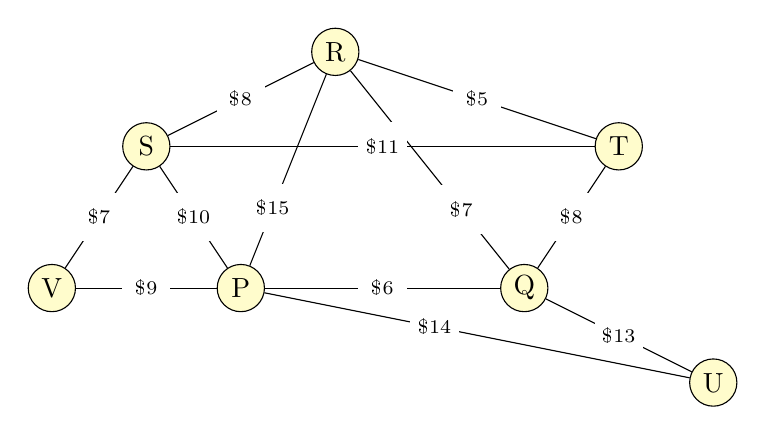
\begin{tikzpicture}[
  scale=1.2,
  every node/.style={circle, draw, fill=yellow!20, minimum size=6mm, inner sep=1pt},
  edge label/.style={font=\scriptsize, rectangle, draw=white, fill=white, inner sep=2pt}
]

% Nodes
\node (P) at (0,0) {P};
\node (Q) at (3,0) {Q};
\node (R) at (1,2.5) {R};
\node (S) at (-1,1.5) {S};
\node (T) at (4,1.5) {T};
\node (U) at (5,-1) {U};
\node (V) at (-2,0) {V};

% Edges with labels
\draw (P) -- (Q) node[midway, edge label] {\$6};
\draw (P) -- (R) node[pos=0.3, edge label] {\$15};
\draw (P) -- (S) node[midway, edge label] {\$10};

\draw (Q) -- (R) node[pos = 0.3, edge label] {\$7};
\draw (Q) -- (T) node[midway, edge label] {\$8};

\draw (R) -- (T) node[midway, edge label] {\$5};
\draw (R) -- (S) node[midway, edge label] {\$8};

\draw (S) -- (T) node[midway, edge label] {\$11};

% New edges
\draw (Q) -- (U) node[midway, edge label] {\$13};
\draw (P) -- (U) node[pos=0.4, edge label] {\$14};
\draw (S) -- (V) node[midway, edge label] {\$7};
\draw (P) -- (V) node[midway, edge label] {\$9};

\end{tikzpicture}


\end{center}

%\vspace{0.5em}
\only<1>{
\begin{algorithm}[H]
\caption{Kruskal's Algorithm}
\begin{boxedminipage}{\linewidth}
\tiny
\begin{algorithmic}[1]
\State \textbf{Input:} A connected, undirected graph $G = (V, E)$ with edge weights $w(e)$.
\State \textbf{Initialization:} Mark all edges as unused. Set $T \gets \emptyset$.
\Repeat
  \State Select the cheapest unused edge in the graph.
  \If{adding the edge would create a cycle}
    \State Skip this edge.
  \Else
    \State Add the edge to $T$.
  \EndIf
\Until{$T$ contains $|V| - 1$ edges (i.e., a spanning tree has been formed).}
\State \textbf{Output:} The set $T$, forming a minimum spanning tree of $G$.
\end{algorithmic}
\end{boxedminipage}
\end{algorithm}
}
\only<2>{
\footnotesize
\begin{tabular}{|c|c|c|c|c|}
\hline
\textbf{Step} & \textbf{Edge Considered} & \textbf{Forms Cycle?}&\textbf{Add to T?} & \textbf{Cost}\\
\hline
1 &  && & \\
\hline
2 &  &  &&\\
\hline
3 &  &  &&\\
\hline
4 &  &  &&\\
\hline
5 &  & && \\
\hline
6 &  & && \\
\hline
7 &  & && \\
\hline
8 &  & && \\
\hline
9 &  &  &&\\
\hline
\end{tabular}
}
\end{frame}





\begin{frame}
The power company needs to lay updated distribution lines connecting the ten Oregon cities below to the power grid.  How can they minimize the amount of new line to lay?
 {\small
\begin{center}
\begin{tabular}{|l|c|c|c|c|c|c|c|c|c|c|}
\hline
&&&&&&&&&&\\[7ex]
& \begin{rotate}{90}Ashland \end{rotate}& \begin{rotate}{90}Astoria\end{rotate}  & \begin{rotate}{90}Bend \end{rotate}& \begin{rotate}{90}Corvallis \end{rotate} & \begin{rotate}{90}Crater Lake \end{rotate} &  \begin{rotate}{90}Eugene  \end{rotate}&  \begin{rotate}{90}Newport \end{rotate} &  \begin{rotate}{90}Portland  \end{rotate}& \begin{rotate}{90}Salem \end{rotate} &  \begin{rotate}{90}Seaside \end{rotate}\\
\hline
Ashland & --&374&200&223&108&178&252&285&240&356\\
\hline
Astoria & 374&--&255&166&433&199&135&95&136&17\\
\hline
Bend & 200 & 255 &--&128&277&128&180 & 160&131&247\\
\hline
Corvalis&223&166&128&--&430&47&52&84&40&155\\
\hline
Crater Lake &108&433&277&430&--&453&478&344&389&423\\
\hline
Eugene &178&199&128&47&453&--&91&110&64&181\\
\hline
Newport&252&135&180&52&478&91&--&114&83&117\\
\hline
Portland &285&95&160&84&344&110&114&--&47&78\\
\hline
Salem & 240 &136&131&40&389&64&83&47&--&118\\
\hline
Seaside&356&17&247&155&423&181&117&78&118&--\\
\hline
\end{tabular}
\end{center}
}
Using Kruskal's algorithm, we add edges from cheapest to most expensive, rejecting any that close a circuit.  We stop when the graph is connected.\\
\end{frame}

\begin{frame}
\vspace{-2cm}
\begin{center}
\begin{tikzpicture}[yscale =0.5, xscale=1.1, every node/.style={font=\tiny}]
\draw[fill] (2,-2) circle[radius=.1] node[below]{Portland};
\draw[fill] (1,0) circle[radius=.1] node[above]{Salem};
\draw[fill] (9,0) circle[radius=.1] node[above]{Corvallis};
\draw[fill] (2,2) circle[radius=.1] node[above]{Seaside};
\draw[fill] (4,3) circle[radius=.1] node[above]{Ashland};
\draw[fill] (4,-3) circle[radius=.1] node[below]{Newport};
\draw[fill] (6,3) circle[radius=.1] node[above]{Astoria};
\draw[fill] (6,-3) circle[radius=.1] node[below]{Eugene};
\draw[fill] (8,2) circle[radius=.1] node[above]{Bend};
\draw[fill] (8,-2) circle[radius=.1] node[below]{Crater Lake};

%\draw[thick, red](1,0)--(9,0);
%\draw[thick, red](1,0)--(2,-2);
%\draw[thick, red](2,2)--(6,3);
%\draw[thick, red](9,0)--(4,-3);
%\draw[thick, red](9,0)--(6,-3);
%\draw[thick, red](8,-2)--(4,3);
%\draw[thick, red](4,3)--(6,-3);
%\draw[thick, red](6,-3)--(8,2);
%\draw[thick, red](2,2)--(2,-2);
\end{tikzpicture}
\end{center}

\end{frame}

\begin{frame}{Extended Example: Oregon Power Grid}
The power company needs to lay distribution lines connecting ten Oregon cities.
\vspace{0.2cm}

\begin{columns}
\begin{column}{0.55\textwidth}
{\small
Cities with shortest connections:
\begin{itemize}
\item Seaside to Astoria: 17 miles
\item Corvallis to Salem: 40 miles
\item Portland to Salem: 47 miles
\item Corvallis to Eugene: 47 miles
\item Corvallis to Newport: 52 miles
\item Portland to Seaside: 78 miles
\item Ashland to Crater Lake: 108 miles
\item Bend to Eugene: 128 miles
\item Eugene to Ashland: 178 miles
\end{itemize}
}
Total: 695 miles of cable
\end{column}

\begin{column}{0.45\textwidth}
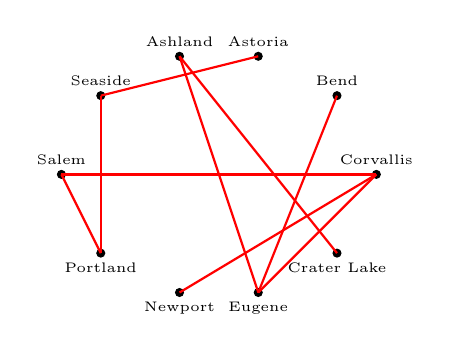
\begin{tikzpicture}[scale=0.5, every node/.style={font=\tiny}]
\draw[fill] (2,-2) circle[radius=.1] node[below]{Portland};
\draw[fill] (1,0) circle[radius=.1] node[above]{Salem};
\draw[fill] (9,0) circle[radius=.1] node[above]{Corvallis};
\draw[fill] (2,2) circle[radius=.1] node[above]{Seaside};
\draw[fill] (4,3) circle[radius=.1] node[above]{Ashland};
\draw[fill] (4,-3) circle[radius=.1] node[below]{Newport};
\draw[fill] (6,3) circle[radius=.1] node[above]{Astoria};
\draw[fill] (6,-3) circle[radius=.1] node[below]{Eugene};
\draw[fill] (8,2) circle[radius=.1] node[above]{Bend};
\draw[fill] (8,-2) circle[radius=.1] node[below]{Crater Lake};

\draw[thick, red](1,0)--(9,0);
\draw[thick, red](1,0)--(2,-2);
\draw[thick, red](2,2)--(6,3);
\draw[thick, red](9,0)--(4,-3);
\draw[thick, red](9,0)--(6,-3);
\draw[thick, red](8,-2)--(4,3);
\draw[thick, red](4,3)--(6,-3);
\draw[thick, red](6,-3)--(8,2);
\draw[thick, red](2,2)--(2,-2);
\end{tikzpicture}
\end{column}
\end{columns}

\end{frame}



\begin{frame}{Key Takeaways}
\begin{itemize}
\item A spanning tree is a connected subgraph with no cycles that includes all vertices
\item A spanning tree of a graph with $n$ vertices always has exactly $n-1$ edges
\item The minimum cost spanning tree (MCST) is the spanning tree with lowest total edge weight
\item Kruskal's algorithm:
  \begin{itemize}
  \item Sort edges by weight
  \item Add edges in order of increasing weight
  \item Skip edges that would create cycles
  \item Stop when you have $n-1$ edges
  \end{itemize}
\item Kruskal's algorithm always produces the optimal solution
\item MCST has applications in network design, infrastructure planning, clustering, and more
\end{itemize}
\end{frame}

\begin{frame}{Prim's Algorithm}
\begin{center}
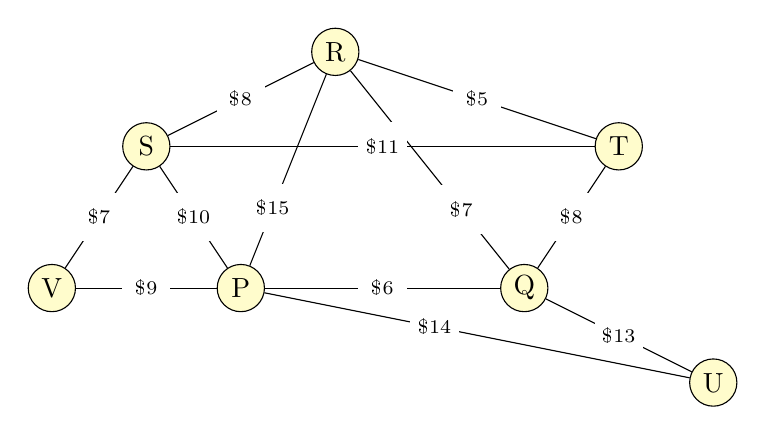
\begin{tikzpicture}[
  scale=1.2,
  every node/.style={circle, draw, fill=yellow!20, minimum size=6mm, inner sep=1pt},
  edge label/.style={font=\scriptsize, rectangle, draw=white, fill=white, inner sep=2pt}
]

% Nodes
\node (P) at (0,0) {P};
\node (Q) at (3,0) {Q};
\node (R) at (1,2.5) {R};
\node (S) at (-1,1.5) {S};
\node (T) at (4,1.5) {T};
\node (U) at (5,-1) {U};
\node (V) at (-2,0) {V};

% Edges with labels
\draw (P) -- (Q) node[midway, edge label] {\$6};
\draw (P) -- (R) node[pos=0.3, edge label] {\$15};
\draw (P) -- (S) node[midway, edge label] {\$10};

\draw (Q) -- (R) node[pos = 0.3, edge label] {\$7};
\draw (Q) -- (T) node[midway, edge label] {\$8};

\draw (R) -- (T) node[midway, edge label] {\$5};
\draw (R) -- (S) node[midway, edge label] {\$8};

\draw (S) -- (T) node[midway, edge label] {\$11};

% New edges
\draw (Q) -- (U) node[midway, edge label] {\$13};
\draw (P) -- (U) node[pos=0.4, edge label] {\$14};
\draw (S) -- (V) node[midway, edge label] {\$7};
\draw (P) -- (V) node[midway, edge label] {\$9};

\end{tikzpicture}


\end{center}

%\vspace{0.5em}
\only<1>{
\begin{algorithm}[H]
\caption{Prim's Algorithm}
\begin{boxedminipage}{\linewidth}
\tiny
\begin{algorithmic}[1]
\State \textbf{Input:} A connected, undirected graph $G = (V, E)$ with edge weights $w(e)$.
\State \textbf{Initialization:} Choose an arbitrary start vertex $v_0 \in V$. Set $T \gets \emptyset$ and $S \gets \{v_0\}$.
\Repeat
  \State From all edges $(u, v)$ where $u \in S$ and $v \notin S$, select the edge with the minimum weight.
  \State Add the selected edge to $T$ and add the new vertex $v$ to $S$.
\Until{$|S| = |V|$ (i.e., all vertices are included).}
\State \textbf{Output:} The set $T$, forming a minimum spanning tree of $G$.
\end{algorithmic}
\end{boxedminipage}
\end{algorithm}
}
\only<2>{
\footnotesize
\begin{tabular}{|c|c|c|c|c|}
\hline
\textbf{Step} & \textbf{Edge Considered} & \textbf{Forms Cycle?}&\textbf{Add to T?} & \textbf{Cost}\\
\hline
1 &  && & \\
\hline
2 &  &  &&\\
\hline
3 &  &  &&\\
\hline
4 &  &  &&\\
\hline
5 &  & && \\
\hline
6 &  & && \\
\hline
7 &  & && \\
\hline
8 &  & && \\
\hline
9 &  &  &&\\
\hline
\end{tabular}
}
\end{frame}

\begin{frame}{Greedy Algorithms for Minimum Spanning Trees}
\textbf{Prim's Algorithm} and \textbf{Kruskal's Algorithm} both solve the \emph{Minimum Spanning Tree (MST)} problem using a \alert{greedy approach}.

\vspace{1em}
\begin{block}{What is a Greedy Algorithm?}
A greedy algorithm builds a solution step-by-step, always choosing the \alert{locally optimal} choice at each step, hoping this leads to a globally optimal solution.
\end{block}

\vspace{1em}
\begin{columns}
\column{0.48\textwidth}
\textbf{Kruskal's Algorithm}
\begin{itemize}
    \item Sorts edges by weight.
    \item Adds the next lightest edge that doesn’t form a cycle.
    \item Builds the MST by connecting components.
\end{itemize}

\column{0.48\textwidth}
\textbf{Prim's Algorithm}
\begin{itemize}
    \item Grows the MST from a starting vertex.
    \item At each step, adds the lightest edge that connects the tree to a new vertex.
\end{itemize}
\end{columns}


\end{frame}

\begin{frame}{Why Do Greedy Algorithms Work for MSTs?}
Minimum Spanning Trees have two key properties that make greedy algorithms like \textbf{Prim's} and \textbf{Kruskal's} provably optimal:

\vspace{1em}
\begin{block}{Greedy-Choice Property}
A globally optimal solution can be arrived at by making a series of locally optimal (greedy) choices.
\begin{itemize}
    \item Choosing the lightest edge never prevents the optimal MST.
    \item Safe edges: The minimum-weight edge crossing any cut must be in some MST.
\end{itemize}
\end{block}

\begin{block}{Optimal Substructure}
An optimal solution to the problem contains within it optimal solutions to subproblems.
\begin{itemize}
    \item Once we select a safe edge, we can recurse on the remaining graph.
    \item The MST is built up piece by piece, maintaining optimality at each step.
\end{itemize}
\end{block}

\vspace{0.5em}
\textit{These properties together ensure that greedy strategies lead to the correct MST.}
\end{frame}


\begin{frame}{Optimality idea}
\textbf{The smallest weight edge must be in a MST}

\begin{center}
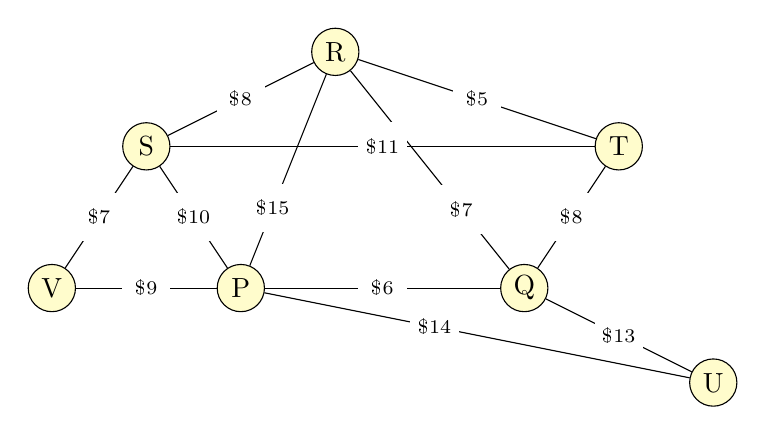
\begin{tikzpicture}[
  scale=1.2,
  every node/.style={circle, draw, fill=yellow!20, minimum size=6mm, inner sep=1pt},
  edge label/.style={font=\scriptsize, rectangle, draw=white, fill=white, inner sep=2pt}
]

% Nodes
\node (P) at (0,0) {P};
\node (Q) at (3,0) {Q};
\node (R) at (1,2.5) {R};
\node (S) at (-1,1.5) {S};
\node (T) at (4,1.5) {T};
\node (U) at (5,-1) {U};
\node (V) at (-2,0) {V};

% Edges with labels
\draw (P) -- (Q) node[midway, edge label] {\$6};
\draw (P) -- (R) node[pos=0.3, edge label] {\$15};
\draw (P) -- (S) node[midway, edge label] {\$10};

\draw (Q) -- (R) node[pos = 0.3, edge label] {\$7};
\draw (Q) -- (T) node[midway, edge label] {\$8};

\draw (R) -- (T) node[midway, edge label] {\$5};
\draw (R) -- (S) node[midway, edge label] {\$8};

\draw (S) -- (T) node[midway, edge label] {\$11};

% New edges
\draw (Q) -- (U) node[midway, edge label] {\$13};
\draw (P) -- (U) node[pos=0.4, edge label] {\$14};
\draw (S) -- (V) node[midway, edge label] {\$7};
\draw (P) -- (V) node[midway, edge label] {\$9};

\end{tikzpicture}


\end{center}
\end{frame}

\begin{frame}{Optimality idea}
\textbf{The smallest weight edge across any cut must be in a MST}

\begin{center}
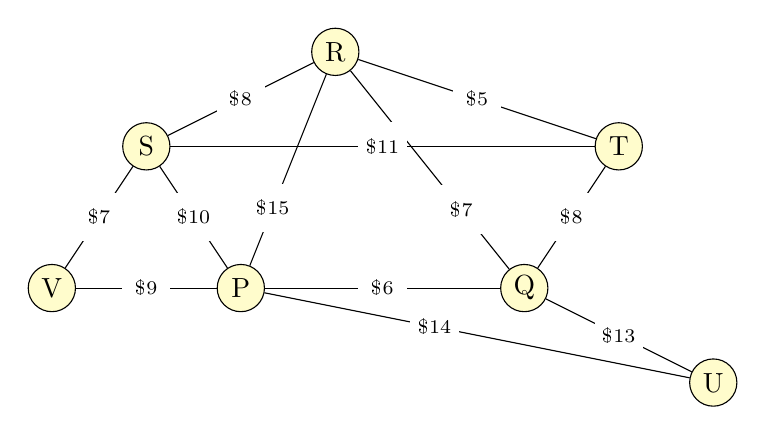
\begin{tikzpicture}[
  scale=1.2,
  every node/.style={circle, draw, fill=yellow!20, minimum size=6mm, inner sep=1pt},
  edge label/.style={font=\scriptsize, rectangle, draw=white, fill=white, inner sep=2pt}
]

% Nodes
\node (P) at (0,0) {P};
\node (Q) at (3,0) {Q};
\node (R) at (1,2.5) {R};
\node (S) at (-1,1.5) {S};
\node (T) at (4,1.5) {T};
\node (U) at (5,-1) {U};
\node (V) at (-2,0) {V};

% Edges with labels
\draw (P) -- (Q) node[midway, edge label] {\$6};
\draw (P) -- (R) node[pos=0.3, edge label] {\$15};
\draw (P) -- (S) node[midway, edge label] {\$10};

\draw (Q) -- (R) node[pos = 0.3, edge label] {\$7};
\draw (Q) -- (T) node[midway, edge label] {\$8};

\draw (R) -- (T) node[midway, edge label] {\$5};
\draw (R) -- (S) node[midway, edge label] {\$8};

\draw (S) -- (T) node[midway, edge label] {\$11};

% New edges
\draw (Q) -- (U) node[midway, edge label] {\$13};
\draw (P) -- (U) node[pos=0.4, edge label] {\$14};
\draw (S) -- (V) node[midway, edge label] {\$7};
\draw (P) -- (V) node[midway, edge label] {\$9};

\end{tikzpicture}


\end{center}
\end{frame}

\begin{frame}{Resources}
\begin{itemize}
\item YouTube Video: "Kruskal's algorithm to find a minimum weight spanning tree" by Kimberly Brehm
\item Additional practice exercises available in the textbook
\end{itemize}

\begin{center}
\Large{Questions?}
\end{center}
\end{frame}

\end{document}